\documentclass{article}
\usepackage[utf8]{inputenc}
\usepackage[margin=1.2in]{geometry}
\usepackage{hyperref}

\usepackage{listings}
\usepackage{xcolor}

\definecolor{codegreen}{rgb}{0,0.6,0}
\definecolor{codegray}{rgb}{0.5,0.5,0.5}
\definecolor{codepurple}{rgb}{0.58,0,0.82}
\definecolor{backcolour}{rgb}{0.95,0.95,0.92}

\lstdefinestyle{mystyle}{
    backgroundcolor=\color{backcolour},   
    commentstyle=\color{codegreen},
    keywordstyle=\color{magenta},
    numberstyle=\tiny\color{codegray},
    stringstyle=\color{codepurple},
    basicstyle=\ttfamily\footnotesize,
    breakatwhitespace=false,         
    breaklines=true,                 
    captionpos=b,                    
    keepspaces=true,                 
    numbers=left,                    
    numbersep=5pt,                  
    showspaces=false,                
    showstringspaces=false,
    showtabs=false,                  
    tabsize=2
}

\lstset{style=mystyle}


\usepackage{tikz}
\usetikzlibrary{positioning}

\usepackage{natbib}
\usepackage{graphicx}
\usepackage{amsmath}

\title{\vspace{-2 cm}Universidade Federal de Ouro Preto \\ PCC104 - Projeto e Análise de Algoritmos \\ Semanas 1 e 2}
\author{Prof. Rodrigo Silva}
%\date{}


\begin{document}

\maketitle


\section{Leitura Recomendada}

\begin{itemize}
    \item Capítulo 2 - \textit{Introduction to the Design and Analysis of Algorithms (3rd Edition)} - Anany Levitin 
\end{itemize}

\section{Questões}

\begin{enumerate}
    
%%%%%%%%%%%%%%%%%%%%%%%%%%%%%%%%%%%%%%%%%%%%%%%%%%%%
%%%%%%%%%%%%%%%%%%%% CAP 2 %%%%%%%%%%%%%%%%%%%%%%%%%
%%%%%%%%%%%%%%%%%%%%%%%%%%%%%%%%%%%%%%%%%%%%%%%%%%%%

    \item Ao que se referem os termos \textit{Complexidade de Tempo} e \textit{Complexidade de Espaço}?
    
    \item Defina os temos, eficiência de melhor caso, caso médio e pior caso.
    
    \item Qual, ou quais os problemas de utilizar unidades de tempo, por exemplo, segundos para analisar o tempo de execução de algoritmos? Qual a a estratégia mais adequada para esta tarefa?
    
    \item Para cada uma das seguintes funções, indique quanto o valor da função aumenta se o tamanho do argumento aumentar 4 vezes.%For each of the following functions, indicate how much the function’s value will change if its argument is increased fourfold.
    
    \begin{enumerate}
        \item $\log_2n$
        \item $\sqrt{n}$
        \item $n$
        \item $n^2$
        \item $n^3$
        \item $2^n$
    \end{enumerate}
    
    \item Eliminação Gaussina é um algoritmo clássico para resolver um sistema de $n$ equações lineares com $n$ variáveis. O método requer aproximadamente $\frac{1}{3}n^3$ multiplicações que é a operação básica do algoritmo.
    \begin{enumerate}
        \item Quantas vezes mais devagar você espera que a resolução de um sistema de 1000 equações seja em relação a um sistema de 500.
        \item Você está considerando comprar 1000 vezes mais rápido do que o seu atual. Por qual fator o novo computador irá aumentar o tamanho dos sistemas resolvíveis no antigo dada a mesma quantidade de tempo? 
    \end{enumerate}
    
    \item Descreva as notações $O$, $\Omega$ e $\Theta$.
    
    \item Prove o seguinte teorema:
    
    \begin{enumerate}
        \item[TEOREMA: ] Se $t_1(n) \in O(g_1(n))$ e $t_2(n) \in O(g_2(n))$ então $ t_1(n) + t_2(n) \in O(\max\{g_1(n),g_2(n)\}) $
    \end{enumerate}
    
    \textit{(OBS: Afirmações análogas são verdadeiras para $\Omega$ e $\Theta$.)}
    
    \item Utilize limites para comparar as seguintes ordens de crescimento:
    \begin{enumerate}
        \item $\frac{1}{2}n(n-1)$ e $n^2$
        \item $\log_2n$ e $\sqrt{n}$
        \item $n!$ e $2^n$
    \end{enumerate}
    
    \item Utilize as definições informais de $O$, $\Omega$ e $\Theta$ para determinar quais das afirmações abaixo são verdadeiras e quais são falsas.
    
    \begin{enumerate}
        \item $n(n+1)/2 \in O(n^3)$
        \item $n(n+1)/2 \in \Theta(n^3)$
        \item $n(n+1)/2 \in O(n^2)$
        \item $n(n+1)/2 \in \Omega(n)$
    \end{enumerate}
    
    
    \item Prove que todo polinômio de grau $k$, $p(n)=a_kn^k + a_{k-1}n^{k-1} + a_{k-2}n^{k-2} ...+ a_0$ com $a_i > 0$, pertence a $\Theta(n^k)$. \textit{(Dica? Você pode provar esta afirmação utilizando limites.)}

    \item Prove que funções exponenciais, $a^n$, têm diferentes ordens de crescimento para diferentes valores da base $a>0$. \textit{(Analise o limite, $\underset{n\rightarrow \infty}{\lim}\frac{a_1^n}{a_2^n}$.)}
    
    %------------Análise algoritmos iterativos 2.3 --------------
    
    \item Considere os três algoritmos abaixo: % 2.3 levitin
    
    \begin{figure}[!ht]
        \centering
        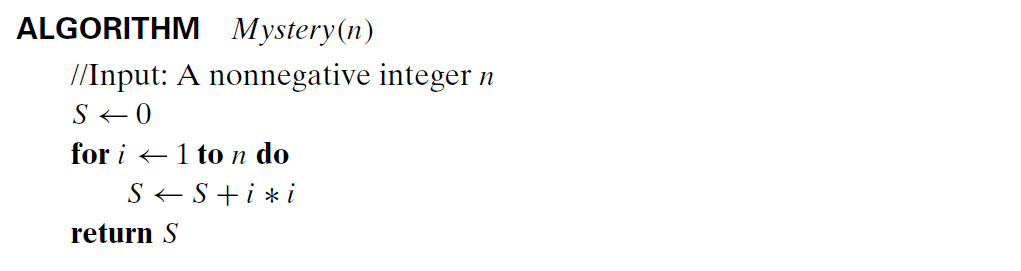
\includegraphics[width=0.6\textwidth]{alg1.PNG}
        \caption{Algoritmo 1}
        \label{fig:alg1}
    \end{figure}
    
    \begin{figure}[!ht]
        \centering
        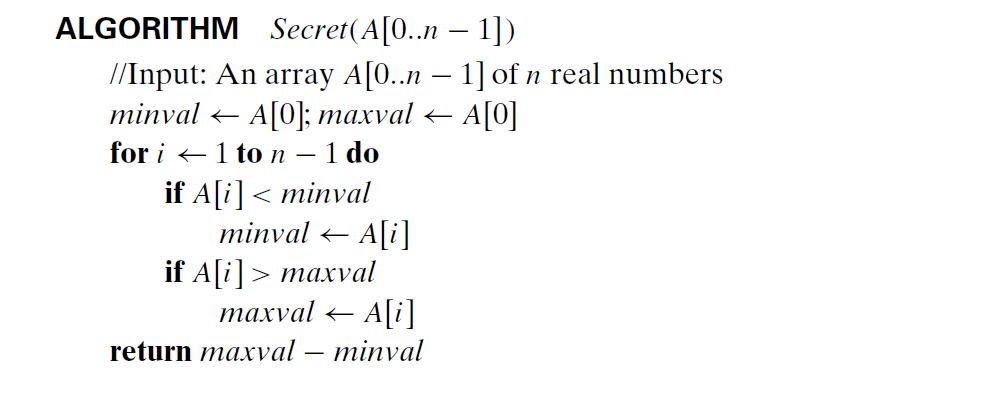
\includegraphics[width=0.6\textwidth]{alg2.PNG}
        \caption{Algoritmo 2}
        \label{fig:alg2}
    \end{figure}
    
    \begin{figure}[!ht]
        \centering
        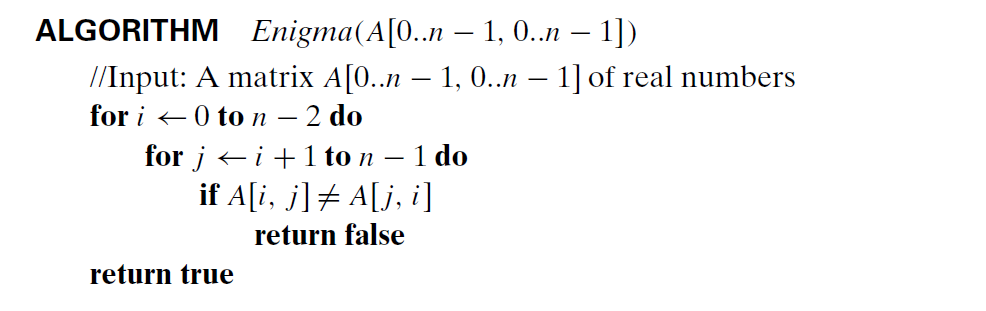
\includegraphics[width=0.6\textwidth]{alg3.PNG}
        \caption{Algoritmo 3}
        \label{fig:alg3}
    \end{figure}
    
    Para cada algoritmo responda:
    \begin{enumerate}
        \item O que este algoritmo computa?
        \item Qual a operação básica deste algoritmo?
        \item Quantas vezes esta operação básica é executada?
        \item Qual a classe deste algoritmo em relação à eficiência?
        \item Sugira alguma melhora ou um novo algoritmo melhor e indique a classe desta sugestão. Se você não conseguir, tente provar que, de fato, a melhora não pode ser feita. 
    \end{enumerate}
    
    % 6. a. Prove that every polynomial of degree k, p(n) = aknk + ak−1nk−1+ . . . + a0 with ak > 0, belongs to (nk).
    % b. Prove that exponential functions an have different orders of growth for different values of base a >0.
    
    % Gaussian eli  mination, the classic algorithm for solving systems of n linear equations in n unknowns, requires about 1 3n3 multiplications, which is the algorithm’s basic operation.
    
    %a) How much longer should you expect Gaussian elimination to work on a system of 1000 equations versus a system of 500 equations?
    
    %b) You are considering buying a computer that is 1000 times faster than the one you currently have. By what factor will the faster computer increase the sizes of systems solvable in the same amount of time as on the old computer? 
    
    %----------- Análise de algoritmos recursivos 2.4 ----------
    \item Resolva as seguintes relações de recorrência:
    \begin{enumerate}
        \item $x(n) = x(n-1) + 5 \text{ para } n>1$, $x(1)=0$
        \item $x(n) = 3x(n-1)\text{ para } n>1$, $x(1)=4$
        \item $x(n) = x(n-1) + n \text{ para } n>0$, $x(0)=0$
        \item $x(n) = x(n/2) + n \text{ para } n>1$, $x(1)=1$ (resolver para $n = 2^k$)
        \item $x(n) = x(n/3) + 1 \text{ para } n>1$, $x(1)=1$ (resolver para $n = 3^k$)
    \end{enumerate}
    
    % Add 8 / 9 / 10
    
    \item Projete um algoritmo para computar $2^n$ para qualquer inteiro não negativo, $n$, baseado na fórmula $2^n = 2^{n-1} + 2^{n-1}$.
    \begin{enumerate}
        \item Apresente a relação de recorrência para o número de adições feitas pelo algoritmo e resolva a relação.
        \item Desenhe a árvore de chamadas recursivas  para este algoritmo e conte o número de chamadas feita pelo algoritmo.
        \item Este é um bom algoritmo para resolver este problema.
    \end{enumerate}
    
    \item Considere o seguinte algoritmo recursivo.
    
    \begin{figure}[!ht]
        \centering
        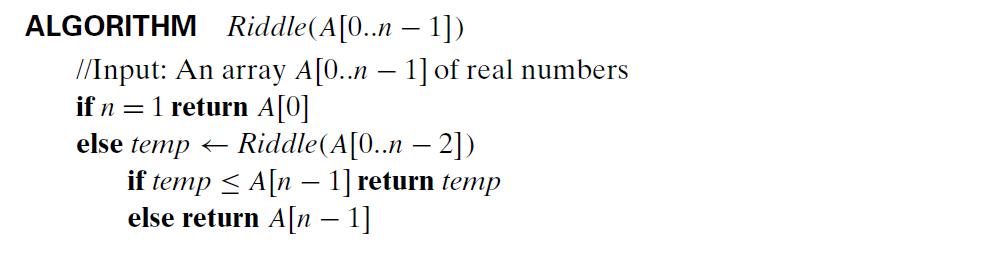
\includegraphics[width=0.8\textwidth]{alg_a.PNG}
        \label{fig:alg_a}
    \end{figure}
    
    \begin{enumerate}
        \item O que este algoritmo faz?
        \item Apresente a relação de recorrência para a operação básica do algoritmo, resolva a relação.
    \end{enumerate}
    
    % -------------- Análise empírica -----------------------
    
    \item Considere o algoritmo abaixo que verifica se um grafo, definido por sua matriz de adjacência é completo. 
    
    \begin{figure}[!ht]
        \centering
        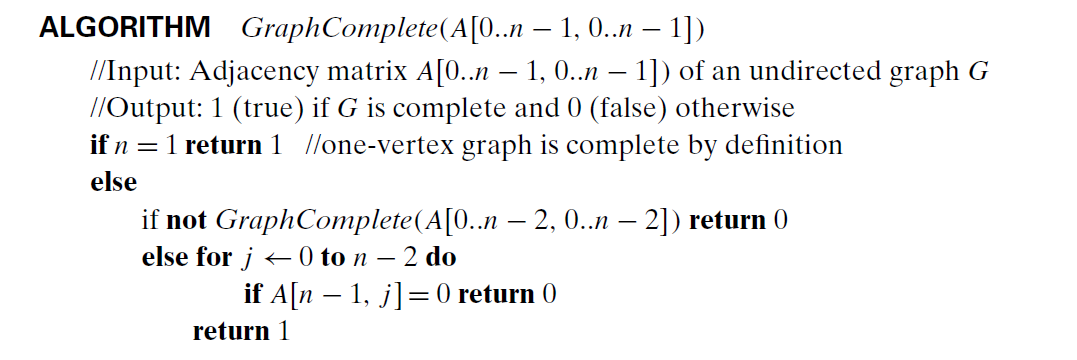
\includegraphics[width=0.8\textwidth]{alg_b.PNG}
        \label{fig:alg_b}
    \end{figure}
    
    Qual é classe de eficiência deste algoritmo no pior caso? 
\end{enumerate}

%\bibliographystyle{plain}
%\bibliography{references}
\end{document}

